% The structural rules of the circuits of Section 6, drawn like
% rule-*.tex: time runs left to right and wire 1 is on top.  A slashed
% wire carries the wires of the box on it or, with no box, any number of
% idle wires.  (shift) is Circuit.Base's cong↑, which adds a wire below;
% (commutation) is its comm₁–comm₃, a gate on the bottom wires against
% any generator placed above it; (involution) and (naturality) are
% Circuit.Prop's σ-inv and σ-nat₁–σ-nat₃.  The last three hold at every
% width with the extra wires on top, hence their idle top wires.
\begin{tabular}{@{}r@{\enspace}l@{\hspace{.8cm}}r@{\enspace}l@{}}
\textup{(shift)} &
$u = v$\enspace$\Longrightarrow$\enspace
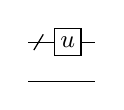
\begin{tikzpicture}[x=1cm,y=1cm,baseline={([yshift=-0.25em]mid)},line width=.45pt]
\coordinate (mid) at (0,-0.250);
\draw (0,0.000)--(0.850,0.000);
\draw (0.070,-0.100)--(0.190,0.100);
\draw (0,-0.500)--(0.850,-0.500);
\draw[fill=white] (0.330,-0.170) rectangle (0.670,0.170);
\node[font=\small] at (0.500,0.000) {$u$};
\end{tikzpicture}%
\xeq
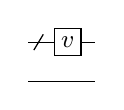
\begin{tikzpicture}[x=1cm,y=1cm,baseline={([yshift=-0.25em]mid)},line width=.45pt]
\coordinate (mid) at (0,-0.250);
\draw (0,0.000)--(0.850,0.000);
\draw (0.070,-0.100)--(0.190,0.100);
\draw (0,-0.500)--(0.850,-0.500);
\draw[fill=white] (0.330,-0.170) rectangle (0.670,0.170);
\node[font=\small] at (0.500,0.000) {$v$};
\end{tikzpicture}%
&
\textup{(commutation)} &
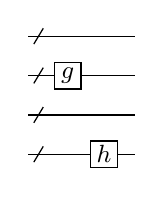
\begin{tikzpicture}[x=1cm,y=1cm,baseline={([yshift=-0.25em]mid)},line width=.45pt]
\coordinate (mid) at (0,-0.750);
\draw (0,0.000)--(1.350,0.000);
\draw (0.070,-0.100)--(0.190,0.100);
\draw (0,-0.500)--(1.350,-0.500);
\draw (0.070,-0.600)--(0.190,-0.400);
\draw (0,-1.000)--(1.350,-1.000);
\draw (0.070,-1.100)--(0.190,-0.900);
\draw (0,-1.500)--(1.350,-1.500);
\draw (0.070,-1.600)--(0.190,-1.400);
\draw[fill=white] (0.330,-0.670) rectangle (0.670,-0.330);
\node[font=\small] at (0.500,-0.500) {$g$};
\draw[fill=white] (0.790,-1.670) rectangle (1.130,-1.330);
\node[font=\small] at (0.960,-1.500) {$h$};
\end{tikzpicture}%
\xeq
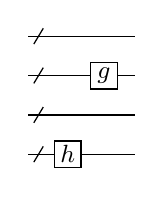
\begin{tikzpicture}[x=1cm,y=1cm,baseline={([yshift=-0.25em]mid)},line width=.45pt]
\coordinate (mid) at (0,-0.750);
\draw (0,0.000)--(1.350,0.000);
\draw (0.070,-0.100)--(0.190,0.100);
\draw (0,-0.500)--(1.350,-0.500);
\draw (0.070,-0.600)--(0.190,-0.400);
\draw (0,-1.000)--(1.350,-1.000);
\draw (0.070,-1.100)--(0.190,-0.900);
\draw (0,-1.500)--(1.350,-1.500);
\draw (0.070,-1.600)--(0.190,-1.400);
\draw[fill=white] (0.330,-1.670) rectangle (0.670,-1.330);
\node[font=\small] at (0.500,-1.500) {$h$};
\draw[fill=white] (0.790,-0.670) rectangle (1.130,-0.330);
\node[font=\small] at (0.960,-0.500) {$g$};
\end{tikzpicture}%
\\\noalign{\vskip 1.8em}
\textup{(involution)} &
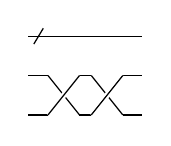
\begin{tikzpicture}[x=1cm,y=1cm,baseline={([yshift=-0.25em]mid)},line width=.45pt]
\coordinate (mid) at (0,-0.500);
\draw (0,0.000)--(1.450,0.000);
\draw (0.070,-0.100)--(0.190,0.100);
\draw (0,-0.500)--(1.450,-0.500);
\draw (0,-1.000)--(1.450,-1.000);
\draw[white,line width=2pt] (0.250,-0.500)--(0.650,-0.500) (0.250,-1.000)--(0.650,-1.000);
\draw (0.250,-0.500)--(0.650,-1.000);
\draw[white,line width=2pt] (0.250,-1.000)--(0.650,-0.500);
\draw (0.250,-1.000)--(0.650,-0.500);
\draw[white,line width=2pt] (0.800,-0.500)--(1.200,-0.500) (0.800,-1.000)--(1.200,-1.000);
\draw (0.800,-0.500)--(1.200,-1.000);
\draw[white,line width=2pt] (0.800,-1.000)--(1.200,-0.500);
\draw (0.800,-1.000)--(1.200,-0.500);
\end{tikzpicture}%
\xeq
\begin{tikzpicture}[x=1cm,y=1cm,baseline={([yshift=-0.25em]mid)},line width=.45pt]
\coordinate (mid) at (0,-0.500);
\draw (0,0.000)--(0.700,0.000);
\draw (0.070,-0.100)--(0.190,0.100);
\draw (0,-0.500)--(0.700,-0.500);
\draw (0,-1.000)--(0.700,-1.000);
\end{tikzpicture}%
&
\textup{(naturality)} &
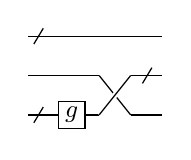
\begin{tikzpicture}[x=1cm,y=1cm,baseline={([yshift=-0.25em]mid)},line width=.45pt]
\coordinate (mid) at (0,-0.500);
\draw (0,0.000)--(1.700,0.000);
\draw (0.070,-0.100)--(0.190,0.100);
\draw (0,-0.500)--(1.700,-0.500);
\draw (0,-1.000)--(1.700,-1.000);
\draw (0.070,-1.100)--(0.190,-0.900);
\draw[fill=white] (0.380,-1.170) rectangle (0.720,-0.830);
\node[font=\small] at (0.550,-1.000) {$g$};
\draw[white,line width=2pt] (0.900,-0.500)--(1.300,-0.500) (0.900,-1.000)--(1.300,-1.000);
\draw (0.900,-0.500)--(1.300,-1.000);
\draw[white,line width=2pt] (0.900,-1.000)--(1.300,-0.500);
\draw (0.900,-1.000)--(1.300,-0.500);
\draw (1.450,-0.600)--(1.570,-0.400);
\end{tikzpicture}%
\xeq
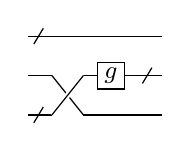
\begin{tikzpicture}[x=1cm,y=1cm,baseline={([yshift=-0.25em]mid)},line width=.45pt]
\coordinate (mid) at (0,-0.500);
\draw (0,0.000)--(1.700,0.000);
\draw (0.070,-0.100)--(0.190,0.100);
\draw (0,-0.500)--(1.700,-0.500);
\draw (0,-1.000)--(1.700,-1.000);
\draw (0.070,-1.100)--(0.190,-0.900);
\draw[white,line width=2pt] (0.300,-0.500)--(0.700,-0.500) (0.300,-1.000)--(0.700,-1.000);
\draw (0.300,-0.500)--(0.700,-1.000);
\draw[white,line width=2pt] (0.300,-1.000)--(0.700,-0.500);
\draw (0.300,-1.000)--(0.700,-0.500);
\draw[fill=white] (0.880,-0.670) rectangle (1.220,-0.330);
\node[font=\small] at (1.050,-0.500) {$g$};
\draw (1.450,-0.600)--(1.570,-0.400);
\end{tikzpicture}%
\end{tabular}%
